\documentclass[a4paper]{article}

\def\npart {III}
\def\nterm {Michaelmas}
\def\nyear {2016}
\def\nlecturer {O. Randal-Williams}
\def\ncourse {Algebraic Topology}
\def\nlectures {MWF.12}

% Imports
\ifx \nextra \undefined
  \usepackage[pdftex,
    hidelinks,
    pdfauthor={Dexter Chua},
    pdfsubject={Cambridge Maths Notes: Part \npart\ - \ncourse},
    pdftitle={Part \npart\ - \ncourse},
  pdfkeywords={Cambridge Mathematics Maths Math \npart\ \nterm\ \nyear\ \ncourse}]{hyperref}
  \title{Part \npart\ - \ncourse}
\else
  \usepackage[pdftex,
    hidelinks,
    pdfauthor={Dexter Chua},
    pdfsubject={Cambridge Maths Notes: Part \npart\ - \ncourse\ (\nextra)},
    pdftitle={Part \npart\ - \ncourse\ (\nextra)},
  pdfkeywords={Cambridge Mathematics Maths Math \npart\ \nterm\ \nyear\ \ncourse\ \nextra}]{hyperref}

  \title{Part \npart\ - \ncourse \\ {\Large \nextra}}
\fi

\author{Lectured by \nlecturer \\\small Notes taken by Dexter Chua}
\date{\nterm\ \nyear}

\usepackage{alltt}
\usepackage{amsfonts}
\usepackage{amsmath}
\usepackage{amssymb}
\usepackage{amsthm}
\usepackage{booktabs}
\usepackage{caption}
\usepackage{enumitem}
\usepackage{fancyhdr}
\usepackage{graphicx}
\usepackage{mathtools}
\usepackage{microtype}
\usepackage{multirow}
\usepackage{pdflscape}
\usepackage{pgfplots}
\usepackage{siunitx}
\usepackage{tabularx}
\usepackage{tikz}
\usepackage{tkz-euclide}
\usepackage[normalem]{ulem}
\usepackage[all]{xy}

\pgfplotsset{compat=1.12}

\pagestyle{fancyplain}
\lhead{\emph{\nouppercase{\leftmark}}}
\ifx \nextra \undefined
  \rhead{
    \ifnum\thepage=1
    \else
      \npart\ \ncourse
    \fi}
\else
  \rhead{
    \ifnum\thepage=1
    \else
      \npart\ \ncourse\ (\nextra)
    \fi}
\fi
\usetikzlibrary{arrows}
\usetikzlibrary{decorations.markings}
\usetikzlibrary{decorations.pathmorphing}
\usetikzlibrary{positioning}
\usetikzlibrary{fadings}
\usetikzlibrary{intersections}
\usetikzlibrary{cd}

\newcommand*{\Cdot}{\raisebox{-0.25ex}{\scalebox{1.5}{$\cdot$}}}
\newcommand {\pd}[2][ ]{
  \ifx #1 { }
    \frac{\partial}{\partial #2}
  \else
    \frac{\partial^{#1}}{\partial #2^{#1}}
  \fi
}

% Theorems
\theoremstyle{definition}
\newtheorem*{aim}{Aim}
\newtheorem*{axiom}{Axiom}
\newtheorem*{claim}{Claim}
\newtheorem*{cor}{Corollary}
\newtheorem*{defi}{Definition}
\newtheorem*{eg}{Example}
\newtheorem*{fact}{Fact}
\newtheorem*{law}{Law}
\newtheorem*{lemma}{Lemma}
\newtheorem*{notation}{Notation}
\newtheorem*{prop}{Proposition}
\newtheorem*{thm}{Theorem}

\renewcommand{\labelitemi}{--}
\renewcommand{\labelitemii}{$\circ$}
\renewcommand{\labelenumi}{(\roman{*})}

\let\stdsection\section
\renewcommand\section{\newpage\stdsection}

% Strike through
\def\st{\bgroup \ULdepth=-.55ex \ULset}

% Maths symbols
\newcommand{\bra}{\langle}
\newcommand{\ket}{\rangle}

\newcommand{\N}{\mathbb{N}}
\newcommand{\Z}{\mathbb{Z}}
\newcommand{\Q}{\mathbb{Q}}
\renewcommand{\H}{\mathbb{H}}
\newcommand{\R}{\mathbb{R}}
\newcommand{\C}{\mathbb{C}}
\newcommand{\Prob}{\mathbb{P}}
\renewcommand{\P}{\mathbb{P}}
\newcommand{\E}{\mathbb{E}}
\newcommand{\F}{\mathbb{F}}
\newcommand{\cU}{\mathcal{U}}
\newcommand{\RP}{\mathbb{RP}}
\newcommand{\CP}{\mathbb{CP}}

\newcommand{\ph}{\,\cdot\,}

\DeclareMathOperator{\sech}{sech}
\DeclareMathOperator{\cosech}{cosech}
\DeclareMathOperator{\cosec}{cosec}

\DeclareMathOperator{\covol}{covol}
\DeclareMathOperator{\vol}{vol}

\let\Im\relax
\let\Re\relax
\DeclareMathOperator{\Im}{Im}
\DeclareMathOperator{\Re}{Re}
\DeclareMathOperator{\im}{im}
\DeclareMathOperator{\image}{image}
\DeclareMathOperator{\Ann}{Ann}

\DeclareMathOperator*{\res}{res}
\DeclareMathOperator{\Res}{Res}
\DeclareMathOperator{\Ind}{Ind}

\DeclareMathOperator{\tr}{tr}
\DeclareMathOperator{\diag}{diag}
\DeclareMathOperator{\rank}{rank}
\DeclareMathOperator{\card}{card}
\DeclareMathOperator{\spn}{span}
\DeclareMathOperator{\adj}{adj}

\DeclareMathOperator{\erf}{erf}
\DeclareMathOperator{\erfc}{erfc}

\DeclareMathOperator{\ord}{ord}
\DeclareMathOperator{\Sym}{Sym}

\DeclareMathOperator{\sgn}{sgn}
\DeclareMathOperator{\orb}{orb}
\DeclareMathOperator{\stab}{stab}
\DeclareMathOperator{\ccl}{ccl}

\DeclareMathOperator{\lcm}{lcm}
\DeclareMathOperator{\hcf}{hcf}

\DeclareMathOperator{\Int}{Int}
\DeclareMathOperator{\id}{id}

\DeclareMathOperator{\betaD}{beta}
\DeclareMathOperator{\gammaD}{gamma}
\DeclareMathOperator{\Poisson}{Poisson}
\DeclareMathOperator{\binomial}{binomial}
\DeclareMathOperator{\multinomial}{multinomial}
\DeclareMathOperator{\Bernoulli}{Bernoulli}
\DeclareMathOperator{\like}{like}

\DeclareMathOperator{\var}{var}
\DeclareMathOperator{\cov}{cov}
\DeclareMathOperator{\bias}{bias}
\DeclareMathOperator{\mse}{mse}
\DeclareMathOperator{\corr}{corr}

\DeclareMathOperator{\otp}{otp}
\DeclareMathOperator{\dom}{dom}

\DeclareMathOperator{\Root}{Root}
\DeclareMathOperator{\supp}{supp}
\DeclareMathOperator{\rel}{rel}
\DeclareMathOperator{\Hom}{Hom}
\DeclareMathOperator{\Aut}{Aut}
\DeclareMathOperator{\Gal}{Gal}
\DeclareMathOperator{\Mat}{Mat}
\DeclareMathOperator{\End}{End}
\DeclareMathOperator{\Char}{char}
\DeclareMathOperator{\ev}{ev}
\DeclareMathOperator{\St}{St}
\DeclareMathOperator{\Lk}{Lk}
\DeclareMathOperator{\disc}{disc}
\DeclareMathOperator{\Isom}{Isom}
\DeclareMathOperator{\length}{length}
\DeclareMathOperator{\energy}{energy}
\DeclareMathOperator{\area}{area}
\DeclareMathOperator{\Syl}{Syl}
\DeclareMathOperator{\cl}{cl}
\DeclareMathOperator{\fix}{fix}

\newcommand{\GL}{\mathrm{GL}}
\newcommand{\SL}{\mathrm{SL}}
\newcommand{\PGL}{\mathrm{PGL}}
\newcommand{\PSL}{\mathrm{PSL}}
\newcommand{\PSU}{\mathrm{PSU}}
\newcommand{\Or}{\mathrm{O}}
\newcommand{\SO}{\mathrm{SO}}
\newcommand{\U}{\mathrm{U}}
\newcommand{\SU}{\mathrm{SU}}

\renewcommand{\d}{\mathrm{d}}
\newcommand{\D}{\mathrm{D}}

\tikzset{->/.style = {decoration={markings,
                                  mark=at position 1 with {\arrow[scale=2]{latex'}}},
                      postaction={decorate}}}
\tikzset{<-/.style = {decoration={markings,
                                  mark=at position 0 with {\arrowreversed[scale=2]{latex'}}},
                      postaction={decorate}}}
\tikzset{<->/.style = {decoration={markings,
                                   mark=at position 0 with {\arrowreversed[scale=2]{latex'}},
                                   mark=at position 1 with {\arrow[scale=2]{latex'}}},
                       postaction={decorate}}}
\tikzset{->-/.style = {decoration={markings,
                                   mark=at position #1 with {\arrow[scale=2]{latex'}}},
                       postaction={decorate}}}
\tikzset{-<-/.style = {decoration={markings,
                                   mark=at position #1 with {\arrowreversed[scale=2]{latex'}}},
                       postaction={decorate}}}

\tikzset{circ/.style = {fill, circle, inner sep = 0, minimum size = 3}}
\tikzset{mstate/.style={circle, draw, blue, text=black, minimum width=0.7cm}}

\definecolor{mblue}{rgb}{0.2, 0.3, 0.8}
\definecolor{morange}{rgb}{1, 0.5, 0}
\definecolor{mgreen}{rgb}{0.1, 0.4, 0.2}
\definecolor{mred}{rgb}{0.5, 0, 0}

\def\drawcirculararc(#1,#2)(#3,#4)(#5,#6){%
    \pgfmathsetmacro\cA{(#1*#1+#2*#2-#3*#3-#4*#4)/2}%
    \pgfmathsetmacro\cB{(#1*#1+#2*#2-#5*#5-#6*#6)/2}%
    \pgfmathsetmacro\cy{(\cB*(#1-#3)-\cA*(#1-#5))/%
                        ((#2-#6)*(#1-#3)-(#2-#4)*(#1-#5))}%
    \pgfmathsetmacro\cx{(\cA-\cy*(#2-#4))/(#1-#3)}%
    \pgfmathsetmacro\cr{sqrt((#1-\cx)*(#1-\cx)+(#2-\cy)*(#2-\cy))}%
    \pgfmathsetmacro\cA{atan2(#2-\cy,#1-\cx)}%
    \pgfmathsetmacro\cB{atan2(#6-\cy,#5-\cx)}%
    \pgfmathparse{\cB<\cA}%
    \ifnum\pgfmathresult=1
        \pgfmathsetmacro\cB{\cB+360}%
    \fi
    \draw (#1,#2) arc (\cA:\cB:\cr);%
}
\newcommand\getCoord[3]{\newdimen{#1}\newdimen{#2}\pgfextractx{#1}{\pgfpointanchor{#3}{center}}\pgfextracty{#2}{\pgfpointanchor{#3}{center}}}

\def\Xint#1{\mathchoice
   {\XXint\displaystyle\textstyle{#1}}%
   {\XXint\textstyle\scriptstyle{#1}}%
   {\XXint\scriptstyle\scriptscriptstyle{#1}}%
   {\XXint\scriptscriptstyle\scriptscriptstyle{#1}}%
   \!\int}
\def\XXint#1#2#3{{\setbox0=\hbox{$#1{#2#3}{\int}$}
     \vcenter{\hbox{$#2#3$}}\kern-.5\wd0}}
\def\ddashint{\Xint=}
\def\dashint{\Xint-}


\begin{document}
\maketitle
{\small
\setlength{\parindent}{0em}
\setlength{\parskip}{1em}

Algebraic Topology assigns algebraic invariants to topological spaces; it permeates modern pure mathematics. This course will focus on (co)homology, with an emphasis on applications to the topology of manifolds. We will cover singular homology and cohomology, vector bundles and the Thom Isomorphism theorem, and the cohomology of manifolds up to Poincar\'e duality. Time permitting, there will also be some discussion of characteristic classes and cobordism, and conceivably some homotopy theory.

\subsubsection*{Pre-requisites}

Basic topology: topological spaces, compactness and connectedness, at the level of Sutherland's book. The course will not assume any knowledge of Algebraic Topology, but will go quite fast in order to reach more interesting material, so some previous exposure to simplicial homology or the fundamental group would be helpful. The Part III Differential Geometry course will also contain useful, relevant material.

Hatcher's book is especially recommended for the course, but there are many other suitable texts.
}
\tableofcontents

\section{Homotopy}
In this course, ``map'' means ``continuous function''.

\begin{defi}[Homotopy]\index{homotopy}
  Let $X, Y$ be a topological space. A \emph{homotopy} between $f_0, f_1: X \to Y$ is a map $F: [0, 1] \times X \to Y$ such that $F(0, x) = f_0(x)$ and $F(1, x) = f_1(x)$. If such an $F$ exists, we say $f_0$ is \emph{homotopic} to $f_1$, and write $f_0 \simeq f_1$.

  This $\simeq$ defines an equivalence relation on the set of maps from $X$ to $Y$.
\end{defi}
This should be thought of as a continuous deformation from $f_0$ to $f_1$. Note that two homotopic functions can be homotopic in several ways.

If we view homotopic functions as ``the same'', then we have to change our respective notion of isomorphism. To do so, we just write down the usual definition of bijection, but with equality replaced with homotopy.

\begin{defi}[Homotopy equivalence]\index{homotopy equivalence}
  A map $f: X \to Y$ is a \emph{homotopy equivalence} if there is some $g: Y \to X$ such that $f \circ g \simeq \id_X$ and $g \circ f \simeq \id_Y$. We call $g$ the \emph{homotopy inverse}\index{homotopy inverse} to $f$.
\end{defi}

\begin{eg}[Stupid example]
  If $f: X \to Y$ is a homeomorphism, then it is a homotopy equivalence --- we take the actual inverse for the homotopy inverse, since equal functions are homotopic.
\end{eg}

\begin{eg}[Interesting example]
  Let $i: \{0\} \to \R^n$ be the inclusion map. To show this is a homotopy equivalence, we have to find a homotopy inverse. Fortunately, there is only one map $\R^n \to \{0\}$, namely the constant function $0$. We call this $r: \R^n \to \{0\}$. The composition $r \circ i: \{0\} \to \{0\}$ is exactly the identity. So this is good.

  In the other direction, the map $r \circ i: \R^n \to \R^n$ sends everything to $0$. We need to produce a homotopy to the identity. We let $F: [0, 1] \to \R^n \to \R^n$ be
  \[
    F(t, \mathbf{v}) = t\mathbf{v}.
  \]
  We have $F(0, \mathbf{v}) = 0$ and $F(1, \mathbf{v}) = \mathbf{v}$. So this is indeed a homotopy from $r \circ i$ to $\id_{\R^n}$.
\end{eg}

So from the point of view of homotopy, the one-point space $\{0\}$ is the same as $\R^n$. So dimension, or even cardinality, is now a meaningless concept. So what is left?

\begin{eg}[Also interesting example]
  Let $S^n \subseteq \R^{n + 1}$ be the unit sphere, and $i: S^n \hookrightarrow \R^{n + 1} \setminus \{0\}$. We show that this is a homotopy equivalence. We define $r: \R^{n + 1} \setminus \{0\} \to S^n$ by
  \[
    r(\mathbf{v}) = \frac{\mathbf{v}}{\|\mathbf{v}\|}.
  \]
  Again, we have $r \circ i = \id_{S^n}$. In the other direction, we need to construct a path from each $\mathbf{v}$ to $\frac{\mathbf{v}}{\|\mathbf{v}\|}$ in a continuous way. We could do so by
  \begin{align*}
    H: [0, 1] \times (\R^{n + 1} \setminus \{0\}) &\to \R^{n + 1} \setminus \{0\}\\
    (t, \mathbf{v}) &\mapsto (1 - t) \mathbf{v} + t \frac{\mathbf{v}}{\|\mathbf{v}\|}.
  \end{align*}
  We can easily check that this is a homotopy from $\id_{\R^{n + 1}\setminus \{0\}}$ to $i \circ r$.
\end{eg}

While dimension is not a meaningful concept in the homotopy world, we can still say something useful about dimensions using homotopies. Suppose we are given that $\R^n \cong \R^m$. Then we know that $\R^n \setminus \{0\} \cong \R^m \{0\}$. Since these are homotopy equivalent to $S^{n - 1}$ and $S^{m - 1}$, this implies that $S^{n - 1} \sim S^{m - 1}$ are homotopy equivalent. We will later show (by calculating homology of both spheres) that this can only happen if $m \not= n$. So by doing some homotopies, we show that dimension is a meaningful concept if we talk about homeomorphism.

We now see a problem in homotopy theory. If we want to show that two spaces are homotopy equivalent, then we just produce a pair of homotopy inverses. The idea is to assign algebraic objects to each topological space that is homotopy invariant. Thus if two spaces are assigned different algebraic objects, then they cannot be homotopy equivalent.

\section{Chain complex}
The first bit of algebra we need is the notion of a chain complex.
\begin{defi}[Chain complex]\index{chain complex}
  A \emph{chain complex} is a sequence of abelian groups and homomorphisms
  \[
    \begin{tikzcd}
      \cdots \ar[r] & C_3 \ar[r, "d_3"] & C_2 \ar[r, "d_2"] & C_1 \ar[r, "d_1"] & C_0 \ar[r, "d_0"] & 0
    \end{tikzcd}
  \]
  such that
  \[
    d_i \circ d_{i + 1} = 0
  \]
  for all $i$.
\end{defi}

Very related to the notion of a chain complex is a \emph{co}chain complex, which is the same thing with the maps the other way.

\begin{defi}[Cochain complex]\index{cochain complex}
  A \emph{cochain complex} is a sequence of abelian groups and homomorphisms
  \[
    \begin{tikzcd}
      0 \ar[r] & C^0 \ar[r, "d^0"] & C^1 \ar[r, "d^1"] & C^2 \ar[r, "d^2"] & C^3 \ar[r] & \cdots
    \end{tikzcd}
  \]
  such that
  \[
    d^{i + 1} \circ d^i = 0
  \]
  for all $i$.
\end{defi}

\begin{defi}[Differentials]\index{differentials}
  The maps $d^i$ and $d_i$ are known as \emph{differentials}.
\end{defi}
Eventually, we will get lazy and just write all the differentials as $d$.

Given a chain complex, the only thing we know is that the composition of any two maps is zero. In other words, we have $\im d_i \subseteq \ker d_{i + 1}$. We can then ask how good this containment is. Is it that $\im d_i = \ker d_{i + 1}$, or perhaps that $\ker d_{i + 1}$ is huge but $\im d_i$ is trivial? The homology or cohomology measures what happens.

\begin{defi}[Homology]\index{homology}
  The \emph{homology} of a chain complex $C_{\Cdot}$ is
  \[
    H_i(C_{\Cdot}) = \frac{\ker (d_i: C_i \to C_{i - 1})}{\im (d_{i + 1}: C_{i + 1} \to C_i)}.
  \]
  An element of $H_i(C_{\Cdot})$ is known as a \term{homology class}.
\end{defi}

Dually, we have
\begin{defi}[Cohomology]\index{cohomology}
  The \emph{cohomology} of a cochain complex $C^{\Cdot}$ is
  \[
    H^i(C^{\Cdot}) = \frac{\ker (d^i: C^i \to C^{i + 1})}{\im (d^{i - 1}: C^{i - 1} \to C^i)}.
  \]
  An element of $H^i(C^{\Cdot})$ is known as a \term{cohomology class}.
\end{defi}

\begin{defi}[Cycles and cocycles]\index{cycle}\index{cocycle}
  The elements of $\ker d_i$ are the \emph{cycles}, and the elements of $\ker d^i$ are the \emph{cocycles}.
\end{defi}

\begin{defi}[Boundaries and coboundaries]\index{boundary}\index{coboundary}
  The elements of $\im d_i$ are the \emph{boundaries}, and the elements of $\im d^i$ are the \emph{coboundaries}.
\end{defi}

So far, this is just algebraic gadgets. We are going to construct chain complexes from topological spaces, and study their (co)homology.

We will define two versions of chain complexes --- one is a really ``big'' one, known as singular (co)chains, which are easy to study formally, but difficult to compute. We will then introduce ``smaller'' ones, which are easy to compute. We will then do some magic to show that they are actually equivalent, which makes us happy.

\section{Singular (co)chains}
\begin{defi}[Standard $n$-simplex]\index{standard $n$-simplex}
  The standard $n$-simplex is
  \[
    \Delta^n = \{(t_0, \cdots, t_n) \in \R^{n + 1} : t_i \geq 0, \sum t_i = 1\}.
  \]
\end{defi}
% insert picture

We notice that $\Delta^n$ has $n + 1$ ``faces''.
\begin{defi}[Face of standard simplex]\index{face of standard simplex}
  The \emph{$i$th face} of $\Delta^n$ is
  \[
    \Delta_i^n = \Delta^n \{(t_0, \cdots, t_n): t_i = 0\}.
  \]
\end{defi}
\begin{center}
  \begin{tikzpicture}
    \draw [->] (-1, 0) -- (3, 0) node [right] {$t_0$};
    \draw [->] (0, -1) -- (0, 3) node [above] {$t_1$};

    \draw (2, 0) -- (0, 2) node [pos=0.5, anchor = south west] {$\Delta_1$};
    \node [circ] at (2, 0) {};
    \node [circ] at (0, 2) {};
    \node at (2, 0) [below] {$\Delta_1^1$};
    \node at (0, 2) [left] {$\Delta_0^1$};
  \end{tikzpicture}
\end{center}
We see that the $i$th face of $\Delta^n$ looks like the standard $n-1$ simplex. Of course, it is just homeomorphic to it, with the map given by
\begin{align*}
  \delta_i: \Delta^{n - 1} &\to \Delta^n\\
  (t_0, \cdots, t_{n - 1}) &\to (t_0, \cdots, t_{i - 1}, 0, t_i, \cdots, t_{n - 1})
\end{align*}
This is a homeomorphism onto $\Delta_i^n$.

\begin{defi}[Singular $n$-simplex]\index{singular $n$-simplex}
  Let $X$ is a space. Then a \emph{singular $n$-simplex} in $X$ is a map $\sigma: \Delta^n \to X$.
\end{defi}

\begin{eg}
  The inclusion of the standard $n$-simplex into $\R^n$ is a singular simplex, but so is the constant map to any point in $X$. So the singular $n$-simplices can be stupid.
\end{eg}

We let $C_n(X)$ be the free abelian group on the set of singular $n$-simplices in $X$. More explicitly, we have
\[
  C_n(X) = \left\{\sum n_\sigma \sigma: \sigma: \Delta^n \to X, n_\sigma \in \Z, \text{only finitely many $n_\sigma$ non-zero}\right\}.
\]
We define $d_n: C_n(X) \to C_{n - 1}(X)$ by
\[
  \sigma \mapsto \sum_{I = 0}^n (-1)^i \sigma \circ \delta_i,
\]
and then extending linearly.

To show this indeed gives a chain complex, we first show the following:
\begin{lemma}
  If $i < j$, then $\delta_j \circ \delta_i = \delta_i \circ \delta_{j - 1} : \Delta^{n - 2} \to \Delta^n$.
\end{lemma}

\begin{proof}
  Both send $(t_0, \cdots, t_{n - 2})$ to $(t_0, \cdots, t_{i - 1}, 0, t_i, \cdots, t_{j - 2}, 0, t_{j - 1}, \cdots, t_{n - 2})$.
\end{proof}

\begin{cor}
  The homomorphism $d_{n - 1} \circ d_n: C_n(X) \to C_{n - 2}(X)$ vanishes.
\end{cor}

\begin{proof}
  It suffices to check this on each basis element $\sigma: \sigma^n \to X$. We have
  \begin{align*}
    d_{n - 1} \circ d_n (\sigma) &= \sum_{i = 0}^{n - 1}(-1)^i \sum_{j = 0}^n (-1)^j \sigma \circ \delta_j \circ \delta_i.
    \intertext{We use the previous lemma to split the sum up into $i < j$ and $i \geq j$:}
    &= \sum_{i < j} (-1)^{i + j} \sigma \circ \delta_j \delta_i + \sum_{i \geq j} (-1)^{i + j} \sigma \circ \delta_j \circ \delta_i\\
    &= \sum_{i < j} (-1)^{i + j} \sigma \circ \delta_i \delta_{j - 1} + \sum_{i \geq j} (-1)^{i + j} \sigma \circ \delta_j \circ \delta_i\\
    &= \sum_{i \leq j} (-1)^{i + j + 1} \sigma \circ \delta_i \circ \delta_j + \sum_{i \geq j} (-1)^{i + j} \sigma \circ \delta_j \circ \delta_i\\
    &= 0.
  \end{align*}
\end{proof}
So the data $d_i: C_n (X) \to d_{i - 1}(X)$ is indeed a chain complex. The only thing we can do to a chain complex is to take its homology!

\begin{defi}[Singular homology]\index{singular homology}
  The \emph{singular homology} of a chain complex $X$ is the homology of the chain complex
  \[
    H_i(X) = H_i(C_{\Cdot}(X), d_{\Cdot}) = \frac{\ker (d_i: C_i(X) \to C_{i - 1}(X))}{ \im(d_{I + 1}: C_{i + 1}(X) \to C_i(X))}.
  \]
\end{defi}
As one might expect, this would be rather hard to compute. Before we do some computations, we construct a ``dual'' version of this as follows:
\begin{defi}[Singular cohomology]\index{singular cohomology}
  We define the dual cochain complex by
  \[
    C^n(X) = \Hom(C_n(X), \Z).
  \]
  We let
  \[
    d^n: C^n(X) \to C^{n + 1}(X)
  \]
  be the adjoint to $d_{n + 1}$, ie.
  \[
    (\varphi: C_n(X) \to \Z) \mapsto (\varphi \circ d_{n + 1}: C_{n + 1}(X) \to \Z).
  \]
  We observe that
  \[
    \begin{tikzcd}
      0 \ar[r] & C^0(X) \ar[r, "d^0"] & C^1(X) \ar[r] & \cdots
    \end{tikzcd}
  \]
  is indeed a cochain complex, since
  \[
    d^{n + 1}(d^n(\varphi)) = \varphi \circ d_{n + 1} \circ d_{n + 2} = \varphi \circ 0 = 0.
  \]
  The \emph{singular cohomology} of $X$ is the cohomology of this cohain complex, ie.
  \[
    H^i(X) = H^i(C^{\Cdot}, d^{\Cdot}) = \frac{\ker(d^i: C^i(X) \to C^{i + 1}(X))}{\im(d^{i - 1}: C^{i - 1}(X) \to C^i (X))}.
  \]
\end{defi}

If we have a space, then we obtain a chain complex like this, which gives us homology groups. What happens to maps between spaces? The object we get is a chain map.

\begin{defi}[Chain map]\index{chain map}
  If $(C_{\Cdot}, d_{\Cdot}^C)$ and $(D_{\Cdot}, d_{\Cdot}^D)$ are chain complexes, then a \emph{chain map} $C_{\Cdot} \to D_{\Cdot}$ is a collection of homomorphism $f_n: C_n \to D_n$ such that $d_n^D \circ f_n = f_{n - 1} \circ d_n^C$. In other words, the following diagram has to commute for all $n$:
  \[
    \begin{tikzcd}
      C_n \ar[r, "f_n"] \ar[d, "d_n^C"] & D_n \ar[d, "d_n^D"]\\
      C_{n - 1} \ar[r, "f_{n - 1}"] & D_{n - 1}
    \end{tikzcd}
  \]
\end{defi}
There is an obvious analogous definition for \term{cochain maps} between cochain complexes.

\begin{lemma}
  If $f_{\Cdot}: C_{\Cdot} \to D_{\Cdot}$ is a chain map, then $f_*: H_n(C_{\Cdot}) \to H_n(D_{\Cdot})$ given by $[x] \mapsto [f_n(x)]$ is a well-defined homomorphism , where $x \in C_n$ is any element representing the homology class $[x] \in H_n(C_{\Cdot})$.
\end{lemma}

\begin{proof}
  Before we check if it is well-defined, we first need to check if it is defined at all! In other words, we need to check if $f_n(x)$ is a cycle. Suppose $x \in C_n$ is a cycle, ie. $d_n^C(x) = 0$. Then we have
  \[
    d_n^D(f_n(x)) = f_{n - 1}(d_n^C(x)) = f_{n - 1}(x) = 0.
  \]
  So $f_n(x)$ is a cycle, and it does represent a homology class.

  To check this is well-defined, if $[x] = [y] \in H_n(C_{\Cdot})$, then $x - y = d_{n + 1}^C(z)$ for some $z$. So $f_n(x) - f_n(y) = f_n d_{n + 1}^C(z) = d_{n + 1}^D (f_{n + 1}(z))$ is a boundary. So we have $[f_n(x)] = [f_n(y)] \in H_n(D_{\Cdot})$.
\end{proof}

\begin{prop}
  If $f: X \to Y$ is a continuous map of topological spaces, then the maps
  \begin{align*}
    f_n: C_n(X) &\to C_n(Y)\\
    (\sigma: \Delta^n \to X) &\mapsto (f \circ \sigma: \Delta^n \to Y)
  \end{align*}
  give a chain map. This induces a map on the homology (and cohomology).
\end{prop}
To see that the $f_n$ and $d_n$ commute, we just notice that $f_n$ acts by composing on the left, and $d_n$ acts by composing on the right, and these two operations commute by the associativity of cuntional composition.

Now if in addition we ahve a map $g: Y \to Z$, then we obtain two maps $H_n(X) \to H_n(Z)$ by
\[
  \begin{tikzcd}
    H_n(X) \ar[rr, "(g \circ f)_*"] \ar[rd, "f_*"] & & H_n(Z)\\
    & H_n(Y) \ar[ru, "g_*"]
  \end{tikzcd}.
\]
By direct inspection of the formula, we see that this diagram commutes. In equation form, we have $(g \circ f)_* = g_* \circ f_*$. Moreover, we have $(\id_X)_* = \id_{H_n(X)}: H_n(X) \to H_n(X)$. Thus we have
\begin{prop}
  If $f: X \to Y$ is a homomeorphism, then $f_*: H_n(X) \to H_n(Y)$ is an isomorphism of abelian groups.
\end{prop}

\begin{proof}
  If $g: Y \to X$ is an inverse to $f$, then $g_*$ is an inverse to $f_*$, as $f_* \circ g_* = (f \circ g)_* = (\id)_* = \id$, and similarly the other way round.
\end{proof}
This is not too exciting. We will later show that \emph{homotopy equivalences} induce isomorphisms of homology groups, which is much harder.

Similarly, applying $\Hom(\ph, \Z)$ to $f_{\Cdot}: C_{\Cdot}(X) \to C_{\Cdot}(Y)$ gives homomorphisms $f^n: C^n(Y) \to C^n(X)$ by mapping $\phi: C_n(Y) \to \Z$ to $\varphi \circ f_n: C_n(X) \to \Z$. Note that this goes the other way!
\[
  \begin{tikzcd}
     C_n(X) \ar[r, "f_n"] & C_n(Y) \ar[r, "\varphi"] & \Z
  \end{tikzcd}
\]
Again, this is a cochain map, and induces maps $f^*: H^n(Y) \to H^n(X)$.

\begin{fact}
  In general, it is \emph{not} true that $H^n(X) = \Hom(H_n(X), \Z)$. Thus, dualizing and taking homology do not commute with each other. However, we will later (hopefully) come up with a relation between the two objects.
\end{fact}

So what does singular homology measure? There are two notions here --- cycles and boundaries.

Suppose we have have a single chain complex $\sigma: \Delta^1 \to X$. Then its boundary $d_1(\sigma) = \sigma(1) - \sigma(0)$. This is in general non-zero, unless we have $\sigma(0) = \sigma(1)$. In other words, this has to be a loop!

% draw diagram with one edge

There can be more ways to obtain cycles. We could have, say, four $1$-simplices $\sigma_1, \sigma_2, \sigma_3, \sigma_4$. In this case we have
\begin{align*}
  \sigma_1(1) &= \sigma_2(0)\\
  \sigma_2(1) &= \sigma_3(0)\\
  \sigma_3(1) &= \sigma_4(0)\\
  \sigma_4(1) &= \sigma_1(0)
\end{align*}
Thus, we have $\sigma_1 + \sigma_2 + \sigma_3 + \sigma_4 \in C_1(X)$. We can view these cycles as detecting the holes by surrounding them. But there are some stupid cycles. % include picture
These are the boundaries. The boundaries also allow us to identify two cycles that surround the same hole, so that we don't double count.
% draw diagram with four edges

\begin{eg}
  We have
  \[
    H^n(\pt) = H_n(\pt) =
    \begin{cases}
      \Z & n = 0\\
      0 & n > 0
    \end{cases}.
  \]
  This is because there is always a single singular $n$-simplex $\sigma_n: \Delta^n \to \pt$. So $C_n(\pt) = \Z$, and is generated by $\sigma_n$. Now note that
  \[
    d_n(\sigma_n) = \sum_{i = 0}^n (-1)^i \sigma_n \delta_i =
    \begin{cases}
      \sigma_{n - 1} & n\text{ even}\\
      0 & n\text{ odd}
    \end{cases}.
  \]
  So the singular chain complex looks like
  \[
    \begin{tikzcd}
      \Z \ar[r, "1"] & \Z\ar[r, "0"] & \Z \ar[r, "1"] & \Z \ar[r, "0"] & \Z \ar[r] & 0.
    \end{tikzcd}
  \]
  The homology groups then follow from direct computation. The cohomology groups are similar.
\end{eg}

\begin{eg}
  If $X = \coprod_{\alpha \in I} X_\alpha$ is a disjoint union of path components, then each singular simplex must lie in some $X_\alpha$. This implies that
  \[
    H_n(X) \cong \bigoplus_{\alpha \in I} H_n(X_\alpha).
  \]
\end{eg}
Now we know how to compute, say, the homology of three points.

\begin{lemma}
  If $X$ is path-connected and non-empty, then $H_0(X) \cong \Z$.
\end{lemma}

\begin{proof}
  Define a homomorphism $\varepsilon: C_0(X) \to \Z$ given by
  \[
    \sum n_\sigma \sigma \mapsto \sum n_\sigma.
  \]
  Then this is surjective. We claim that the composition
  \[
    \begin{tikzcd}
      C_1(X) \ar[r, "d"] & C_0(x) \ar[r, "\varepsilon"] & \Z
    \end{tikzcd}
  \]
  is zero. Indeed, each simplex has two ends, annd a $\sigma: \Delta^1 \to X$ is mapped to $\sigma \circ \delta_0 - \sigma \circ \delta_1$, which is mapped by $\varepsilon$ to $1 - 1 = 0$.

  Thus, we obtain a well-defined map $\varepsilon: H_0(X) \to \Z$ mapping $[x] \mapsto \varepsilon(x)$, and is surjective.

  So far, this is true for a general space. Now suppose $\sum n_\sigma \sigma \in C_0(X)$ lies in $\ker \varepsilon$. We choose an $x_0 \in X$. As $X$ is path-conected, for each of $\Delta^0 \to X$ we can choose a path $\tau_\sigma: \Delta^1 \to X$ with $\tau_\sigma \circ \delta_0 = \sigma$ and $\tau_\sigma \circ \delta_1 = x_0$.

  Given these $1$-simplices, we can form a $1$-chain $\sum n_\sigma \tau_\sigma \in C_1(X)$, and
  \[
    d_1\left(\sum n_\sigma \tau_\sigma\right)= \sum n_\sigma(\sigma + x_0) = \sum n_\sigma \cdot \sigma - \left(\sum n_\sigma\right) x_0.
  \]
  Now we use the fact that $\sum n_\sigma = 0$. So $\sum n_\sigma \cdot \sigma$ is a boundary. So it is zero in $H_0(X)$.
\end{proof}

Combining with the coproduct formula, we have
\begin{prop}
  For any space $X$, we have $H_0(X)$ is a free abelian group generated by the path components of $X$.
\end{prop}
These are pretty much the things we can do by hand. To do more things, we need to use some tools. We will first state them and use them, and leave the proof for a later time.

\section{Four major tools of (co)homology}
\subsection{Homotopy invariance}
\begin{thm}[Homotopy invariance theorem]\index{homotopy invariance theorem}
  Let $f \simeq g: X \to Y$ be homotopic maps. Then
  \[
    f_* = g_*: H_{\Cdot}(X) \to H_{\Cdot}(Y)
  \]
  and
  \[
    f^* = g^* = H^{\Cdot}(X) \to H^{\Cdot}(Y).
  \]
\end{thm}

\begin{cor}
  If $f: X \to Y$ is a homotopy equivalence, then $f_*: H_{\Cdot}(X) \to H_{\Cdot}(Y)$ and $f^*: H^{\Cdot}(X) \to H^{\Cdot}(Y)$ are isomorphisms.
\end{cor}

\begin{proof}
  If $g: Y \to X$ is a homotopy inverse, then
  \[
    g_* \circ f_* = (g \circ f)_* = (\id_X)_* = \id_{H_{\Cdot}(X)}.
  \]
  Similarly, we have $f_* \circ g_* = (\id_Y)_* = \id_{H_{\Cdot}(Y)}$. So $f_*$ is an isomorphism when an inverse of $g_*$.

  The case for cohomology is similar.
\end{proof}

\begin{eg}
  We have
  \[
    H^n(\R^n) = H_n(\R^n) =
    \begin{cases}
      \Z & n = 0\\
      0 & n > 0
    \end{cases}.
  \]
\end{eg}

The next tool is something that allows us to compute (co)homology by computing the (co)homology of smaller subspaces. Before we do that, we need to introduce an algebraic notion.

\subsection{Mayer-Vietoris}
\begin{defi}[Exact sequence]\index{exact sequence}
  We say homomorphisms
  \[
    \begin{tikzcd}
      A \ar[r, "f"] & B \ar[r, "g"] & C
    \end{tikzcd}
  \]
  is \emph{exact at $B$} if $\im(F) = \ker(G)$.

  We say a sequence
  \[
    \begin{tikzcd}
      \cdots \ar[r] & X_0 \ar[r] & X_1 \ar[r] & X_2 \ar[r] & \cdots
    \end{tikzcd}
  \]
  is \emph{exact} if it is exact at each $X_n$.
\end{defi}

\begin{eg}
  If
  \[
    \begin{tikzcd}
      0 \ar[r] & A \ar[r, "f"] & B \ar[r] & 0
    \end{tikzcd}.
  \]
  is exact, then $f$ is an isomorphism.
\end{eg}

\begin{defi}[Short exact sequence]\index{short exact sequence}
  A \emph{short exact sequence} is a sequence of the form
  \[
    \begin{tikzcd}
      0 \ar[r] & A \ar[r] & B \ar[r] & C \ar[r] & 0
    \end{tikzcd}.
  \]
\end{defi}

\begin{lemma}
  In a short exact sequence
  \[
    \begin{tikzcd}
      0 \ar[r] & A \ar[r, "f"] & B \ar[r, "g"] & C \ar[r] & 0
    \end{tikzcd},
  \]
  the map $f$ is injective; $g$ is surjective, and $C \cong B/A$.
\end{lemma}

\begin{eg}
  Consider the sequence
  \[
    \begin{tikzcd}
      0 \ar[r] & \Z/n\Z \ar[r] & A \ar[r] & \Z/m\Z \ar[r] & 0
    \end{tikzcd}
  \]
  There are many possible values of $A$. A few obvious examples are $A = \Z/nm\Z$ and $A = \Z/n\Z \oplus \Z/m\Z$. If $n$ and $m$ are not coprime, then these are different groups.
\end{eg}
Many of the important theorems for computing homology groups tell us that the homology groups of certain spaces fall into some exact sequence, and we have to try figure out what the groups are.

\begin{thm}[Mayer-Vietoris theorem]\index{Mayer-Vietoris theorem}
  Let $X = A \cup B$ be the union of two open subsets. We have inclusions
  \[
    \begin{tikzcd}
      A \cup B \ar[r, "i_A", hook] \ar[d, "i_B", hook] & A \ar[d, hook, "j_A"]\\
      B \ar[r, hook, "j_B"] & X
    \end{tikzcd}.
  \]
  Then there are homomorphisms $\partial_{MV}: H_n(X) \to H_{n - 1}(A \cap B)$ such that the following sequence is exact:
  \[
    \begin{tikzcd}
      \cdots \ar[r, "\partial_{MV}"] & H_n(A \cap B) \ar[r, "i_{A*} \oplus i_{B*}"] & H_n(A) \oplus H_n(B) \ar[r, "j_{A*} - j_{B*}"] & H_n(X)\ar[out=0, in=180, looseness=2, overlay, lld, "\partial_{MV}"']\\
      & H_{n - 1}(A \cap B) \ar[r, "i_{A*} \oplus i_{B*}"] & H_{n - 1}(A) \oplus H_{n - 1}(B) \ar[r, "j_{A*} - j_{B*}"] & H_{n - 1}(X) \ar [r] & \cdots\\
      &\cdots \ar[r] & H_0(A) \oplus H_0(B) \ar[r, "j_{A*} - j_{B*}"] & H_0(X) \ar [r] & 0
    \end{tikzcd}
  \]
  Furthermore, the Mayer-Vietoris sequence is \emph{natural}, ie. if $f: X = A\cup B \to Y = U \cup V$ satisfies $f(A) \subseteq U$ and $f(B) \subseteq V$, then the diagram
  \[
    \begin{tikzcd}
       H_{n + 1}(X) \ar[r, "\partial_{MV}"] \ar[d, "f_*"] & H_{n}(A \cap B) \ar[r, "i_{A*} \oplus i_{B*}"] \ar[d, "f|_{A \cap B*}"] & H_n(A) \oplus H_n(B) \ar[r, "j_{A*} - j_{B*}"] \ar[d, "f|_{A*} \oplus f|_{B*}"] & H_n(X) \ar[d, "f_*"]\\
       H_{n + 1}(Y) \ar[r, "\partial_{MV}"] & H_{n}(U \cap V) \ar[r, "i_{U*} \oplus i_{V*}"] & H_n(U) \oplus H_n(V) \ar[r, "j_{U*} - j_{V*}"] & H_n(Y)
    \end{tikzcd}
  \]
  commutes.
\end{thm}
For certain elements of $H_{n + 1}(X)$, we can easily specify what $\partial_{MV}$ does to it. The meat of the proof is to show that every element of $H_{n + 1}(X)$ can be made to look like that.

Indeed, if $[a + b] \in H_n(X)$ is such that $a \in C_n(A)$ and $b \in C_n(B)$, then we have
\[
  \partial_{MV}([a + b]) = [d_n(a)] = [-d_n(b)] \in H_n(A \cap B).
\]
To see this makes sense, note that we have $d_n(a + b) = 0$. So $d_n(a) = - d_n(b)$. Moreover, since $a \in C_n(A)$, we have $d_n(a) \in C_{n - 1}(A)$. Similarly, $d_n(b) \in C_{n - 1}(B)$. So $d_n(a) = - d_n(b) \in C_n(A) \cap C_n(B) = C_n(A \cap B)$.

\subsection{Relative homology}
The next tool involves relative homology.
\begin{defi}[Relative homology]\index{relative homology}
  Let $A \subseteq X$. We write $i: A \to X$ for the inclusion map. Then the map $i_n: C_n(A) \to C_n(X)$ is injective as well, and we write
  \[
    C_n(X, A) = \frac{C_n(X)}{C_n(A)}.
  \]
  The differential $d_n: C_n(X) \to C_{n - 1}(X)$ restricts to a map $C_n(A) \to C_{n - 1}(A)$, and thus gives a well-defined differential $d_n: C_n(X, A) \to C_{n - 1}(X, A)$, sending $[c] \mapsto [d_n(c)]$. So we write
  \[
    H_n(X, a) = H_n(C_{\Cdot}(X, A)).
  \]
\end{defi}
We think of this as chains in $X$ where we ignore everything that happens in $A$.

\begin{thm}[Exact sequence for relative homology]\index{exact sequence for relative homology}
  There are homomorphisms $\partial: H_n(X, A) \to H_{n - 1}(A)$ given by mapping
  \[
    \big[[c]\big] \mapsto [d_n c].
  \]
  This makes sense because $c \in C_n(x)$, so $[c] \in C_n(X)/C_n(A)$. We know $[d_n c] = 0 \in C_{n - 1}(X)/C_{n - 1}(A)$. So $d_n c \in C_{n - 1}(A)$. So this notation makes sense.

  Moreover, there is a long exact sequence
  \[
    \begin{tikzcd}
      \cdots \ar[r, "\partial"] & H_n(A) \ar[r, "i_*"] & H_n(X) \ar[r, "q_*"] & H_n(X, A)\ar[out=0, in=180, looseness=2, overlay, lld, "\partial"']\\
      & H_{n - 1}(A) \ar[r, "i_*"] & H_{n - 1}(X) \ar[r, "q_*"] & H_{n - 1}(X, A) \ar [r] & \cdots\\
      &\cdots \ar[r] & H_0(X) \ar[r, "q_*"] & H_0(X, A) \ar [r] & 0
    \end{tikzcd},
  \]
  where $i_*$ is induced by $i: C_{\Cdot}(A) \to C_{\Cdot}(X)$ and $q_*$ is induced by the quotient $q: C_{\Cdot}(X) \to C_{\Cdot}(X, A)$.
\end{thm}

\begin{defi}[Map of pairs]\index{map of pairs}
  Let $(X, A)$ and $(Y, B)$ be topological spaces with $A \subseteq X$ and $B \subseteq Y$. A \emph{map of pairs} is a map $f: X \to Y$ such that $f(A) \subseteq B$.
\end{defi}

Such a map induces a map $f_*: H_n(X, A) \to H_n(Y, B)$, and the exact sequence for relative homology is natural for such maps.

\subsection{Excision theorem}
The main point of relative homology is that we want to think of $H_n(X, A)$ as the homology of $X$ when we ignore $A$. However, it is not true in general that, say, $H_n(X, A) = H_n(X \setminus A)$. However, we are allowed to remove subspaces of $A$ that are ``not too big'', as specified by the excision theorem:

\begin{thm}[Excision theorem]\index{excision theorem}
  Let $X(, A)$ be a pair of spaces, and $Z \subseteq A$ be such that $\overline{Z} \subseteq \mathring{A}$. Then the map
  \[
    H_n(X \setminus Z, A \setminus Z) \to H_n(X, A)
  \]
  is an isomorphism.
\end{thm}
% insert picture

While we've only been talking about homology, everything so far holds analogously for cohomology too. It is again homotopy invariant, and there is a Mayer-Vietoris sequence (with maps $\partial_{MV}: H^n(A \cap B) \to H^{n + 1}(X)$). The relative cohomology is defined by $C^{\Cdot}(X, A) = \Hom(C_{\Cdot}(X, A), \Z)$ and so $H^*(X, A)$ is the cohomology of that. Similarly, excision holds.

\subsection{Applications}
\begin{eg}
  Consider the space $S^1$. We can split $S^1$ up as
  \begin{center}
    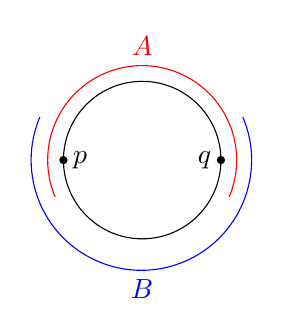
\begin{tikzpicture}
      \draw circle [radius=1];
      \draw [red] (1.105, -0.4673) arc(-22.9:202.9:1.2);
      \node [red, above] at (0, 1.2) {$A$};

      \draw [blue] (1.279, 0.545) arc(22.9:-202.9:1.4);
      \node [blue, below] at (0, -1.4) {$B$};

      \node [circ] at (1, 0) {};
      \node at (1, 0) [left] {$q$};
      \node [circ] at (-1, 0) {};
      \node at (-1, 0) [right] {$p$};
    \end{tikzpicture}
  \end{center}
  We want to apply Mayer-Vietoris. We have
  \[
    A \cong B \cong \R \simeq *,\quad A \cap B \cong \R \coprod \R \simeq \{p\} \coprod \{q\}.
  \]
  We obtain
  \[
    \begin{tikzcd}
      \cdots \ar[r] & H_1(A \cap B) \ar[r] & H_1(A) \oplus H_1(B) \ar[r] & H_1(S^1)\ar[out=0, in=180, looseness=2, overlay, lld]\\
      & H_0(A \cap B) \ar[r, "i_{A*} \oplus i_{B*}"] & H_0(A) \oplus H_0(B) \ar[r] & H_0(S^1) \ar [r] & 0
    \end{tikzcd}
  \]
  We replace these with the known objects to get
  \[
    \begin{tikzcd}
      \cdots \ar[r] & 0 \ar[r] & 0 \ar[r] & H_1(S^1)\ar[out=0, in=180, looseness=2, overlay, lld, "f"]\\
      & \Z \oplus \Z \ar[r, "g"] & \Z \oplus \Z \ar[r] & \Z \ar [r] & 0
    \end{tikzcd}
  \]
  We can now try to figure out what the maps are. We know that $H_0(A \cap B) \cong \Z \oplus \Z$ is generated by $p$ and $q$, and the inclusion map sends each of $p$ and $q$ to the unique connected components of $A$ and $B$. So the homology classes are both sent to $(1, 1) \in H_0(A) \oplus H_0(B) \cong \Z \oplus \Z$. We then see that the kernel of $g$ is generated by $(p - q)$, and is thus isomorphic to $\Z$.

  Since the map into $H_1(S^1)$ is from $0$, it has trivial image. So the map $f$ must be injective by exactness. So $H_1(S^1)$ is isomorphic to its image in $H_0(A \cap B)$ The image of $f$ is the kernel of $g$, and is thus isomorphic to $\Z$.

  By looking higher up the exact sequence, we see that all other homology groups vanish.
\end{eg}

We can do the sphere in general in the same way.

\begin{thm}
  For any $n \geq 1$, we have
  \[
    H_i(S^n) =
    \begin{cases}
      \Z & i = 0, n\\
      0 & \text{otherwise}
    \end{cases}.
  \]
\end{thm}

\begin{proof}
  We cut up $^n$ as
  \begin{align*}
    A &= S^n \setminus \{N\} \cong \R^n \simeq *,\\
    B &= S^n \setminus \{S\} \cong \R^n \simeq *,
  \end{align*}
  where $N$ and $S$ are the north and south poles. Moreover, we have
  \[
    A\cap B \cong \R \times S^{n - 1} \simeq S^{n - 1}
  \]
  So we can ``induct up'' using the Mayer-Vietoris sequence:
  \[
    \begin{tikzcd}
      \cdots \ar[r] & H_i(S^{n - 1}) \ar[r] & H_i(*) \oplus H_i(*) \ar[r] & H_i(S^n)\ar[out=0, in=180, looseness=2, overlay, lld, "\partial"]\\
      & H_{i - 1}(S^{n - 1}) \ar[r] & H_{i - 1}(*) \oplus H_{i - 1}(*) \ar[r] & H_{i - 1}(S^n) \ar [r] & \cdots
    \end{tikzcd}
  \]
  Now suppose $n \geq 2$, as we already did $S^1$ already. If $i > 1$, then $H_1(*) = 0 = H_{i - 1}(*)$. So the Mayer-Vietoris map
  \[
    \begin{tikzcd}
      H_i(S^n) \ar[r, "\partial"] & H_{i - 1}(S^{n - 1})
    \end{tikzcd}
  \]
  is an isomorphism.

  All that remains is to look at $i = 0, 1$. The $i = 0$ case is trivial. For $i = 1$, we look at
  \[
    \begin{tikzcd}
      & \cdots \ar[r] & H_1(*) \oplus H_1(*) \ar[r] & H_1(S^n)\ar[out=0, in=180, looseness=2, overlay, lld, "\partial"]\\
      & H_0(S^{n - 1}) \ar[r] & H_0(*) \oplus H_0(*) \ar[r] & H_0(S^n) \ar [r] & 0
    \end{tikzcd}
  \]
  Again, we plug in the known values to obtain
  \[
    \begin{tikzcd}
      & \cdots \ar[r] & 0 \ar[r] & H_1(S^n)\ar[out=0, in=180, looseness=2, overlay, lld]\\
      & \Z \ar[r, "f"] & \Z \oplus \Z \ar[r] & \Z \ar [r] & 0
    \end{tikzcd}
  \]
  To conclude that $H_1(S^n)$ is trivial, it suffices to show that the map $f$ is injective. But picking the canonical generators, it is given by $1 \mapsto (1, 1)$.
\end{proof}
While we know what the groups are, it is difficult for us to figure out what the generators of the groups are, since we need to trace through lots of Mayer-Vietoris homomorphisms. Later, we will develop cellular homology, which will make this much easier.

\begin{cor}
  If $n \not= m$, then $S^{n - 1} \not\simeq S^{m - 1}$, since they have different homology groups.
\end{cor}

\begin{cor}
  If $n \not= m$, then $\R^n \not \cong \R^m$.
\end{cor}

We can also use homology to define a useful notion.
\begin{defi}[Degree of a map]\index{degree of map}
  Let $f: S^n \to S^n$ be a map. Then we obtain a map $f_*: H_n(S^n) \to H_n(S^n)$. But we know $H_n(S^n) \cong \Z$. We know that any map from $\Z$ to itself is multiplication by an integer, which we call the \emph{degree} of $f$, written $\deg(f)$.
\end{defi}

In particular, for $n = 1$, the degree is the winding number.

Elementary properties of the degree follows from properties of homology.
\begin{prop}\leavevmode
  \begin{enumerate}
    \item $\deg(\id_{S^n}) = 1$.
    \item If $f$ is not surjective, then $\deg(f) = 0$.
    \item Homotopic maps have equal degrees.
  \end{enumerate}
\end{prop}

\begin{proof}\leavevmode
  \begin{enumerate}
    \item Obvious.
    \item If $f$ is not surjective, then $f$ can be factored as
      \[
        \begin{tikzcd}
          S^n \ar[r, "f"] & S^n \setminus \{p\} \ar[r, hook] & S^n
        \end{tikzcd},
      \]
      where $p$ is some point not in the image of $f$. But $S^n \setminus \{p\}$ is contractible. So $f_*$ factors as
      \[
        \begin{tikzcd}
          f_*: H_n(S^n) \ar[r] & H_n(*) = 0 \ar[r] & H_n(S^n)
        \end{tikzcd}.
      \]
      So $f_*$ is the zero homomorphism, and is thus multiplication by $0$.
    \item Obvious as well.
  \end{enumerate}
\end{proof}

\printindex
\end{document}
